




%%%%%%% GPUs: Disillusion %%%%%%%

\begin{frame}{Hardware Specifications}
 \begin{block}{Peak FLOP/s} \end{block}
 \begin{center} \vspace*{-0.9cm} 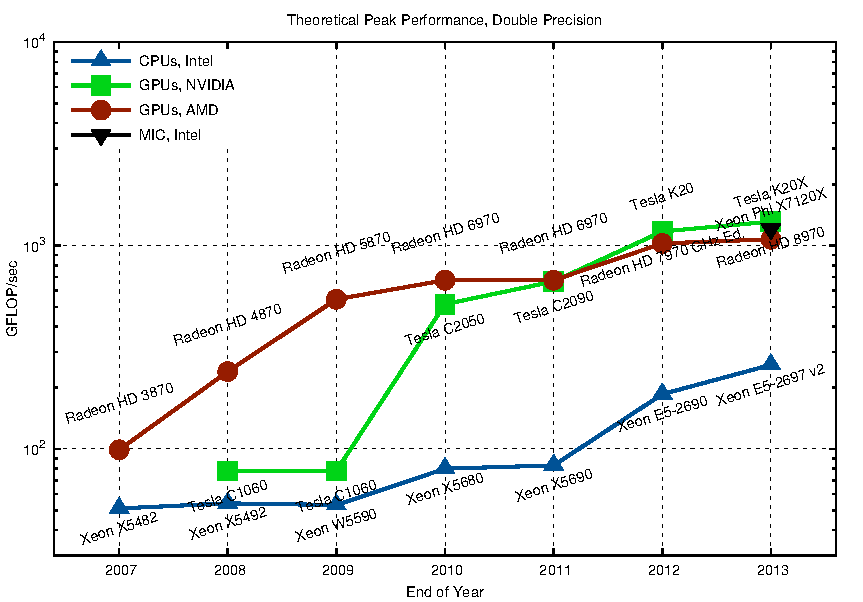
\includegraphics[width=0.95\textwidth]{figures/gflops-dp} \end{center}
\end{frame}

\begin{frame}{Hardware Specifications}
 \begin{block}{Peak Memory Bandwidth} \end{block}
 \begin{center} \vspace*{-0.9cm} 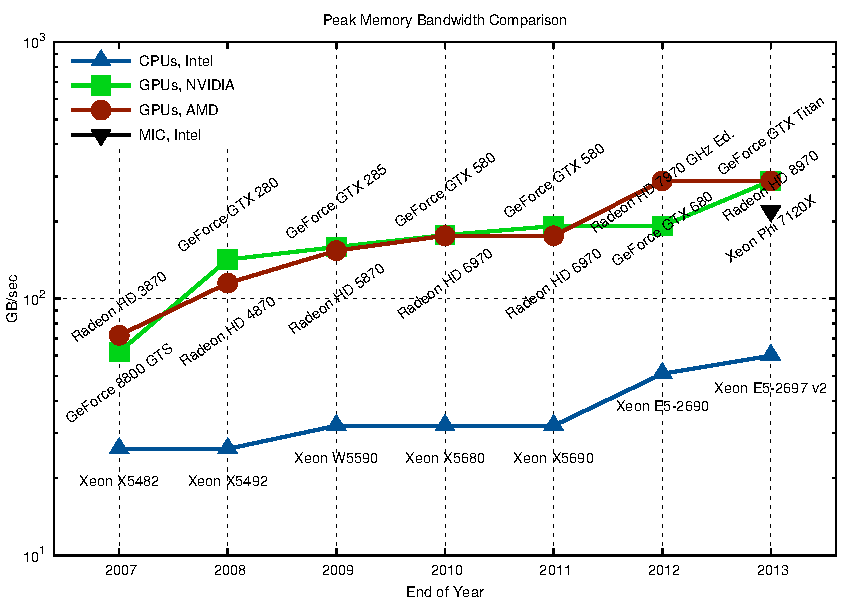
\includegraphics[width=0.95\textwidth]{figures/mem-bw} \end{center}
\end{frame}

\begin{frame}{Hardware Specifications}
 \begin{block}{FLOPs/Byte} \end{block}
 \begin{center} \vspace*{-0.9cm} 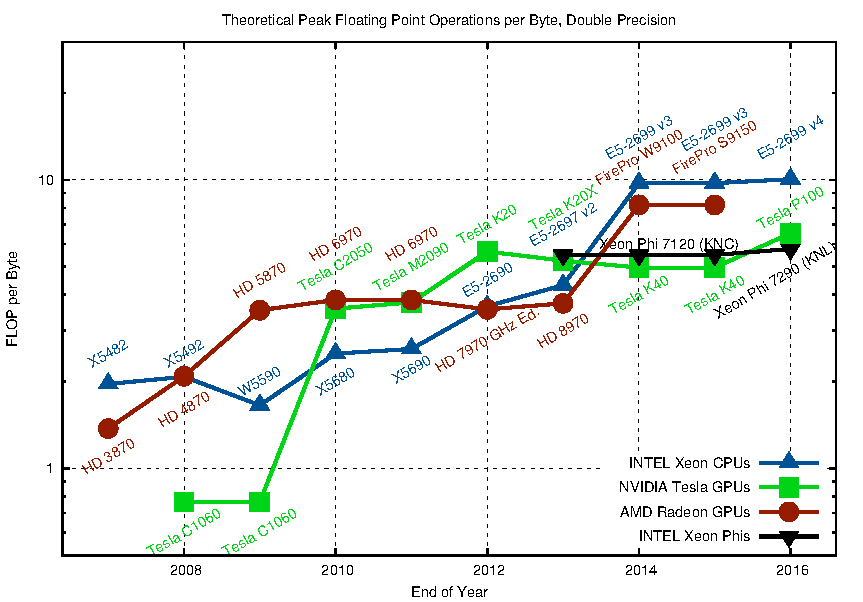
\includegraphics[width=0.95\textwidth]{figures/flop-per-byte-dp} \end{center}
\end{frame}

\begin{frame}{GPUs: Disillusion}
 \begin{center} 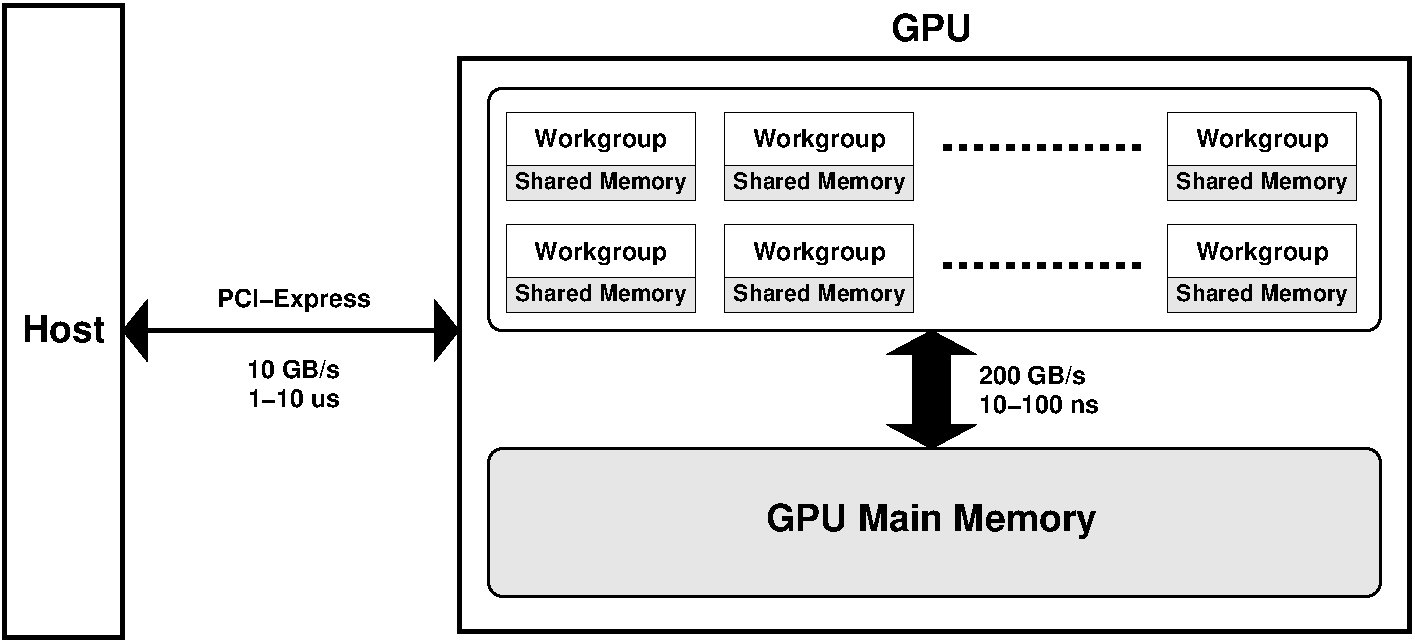
\includegraphics[width=0.99\textwidth]{figures/gpu-schematic} \end{center}
\end{frame}






\begin{frame}[fragile]
\frametitle{Comparison with CUDA and OpenACC}
 \begin{block}{NVIDIA CUDA}
  \begin{lstlisting}
// GPU kernel:
__global__ void kernel(double *buffer)
{
  int idx = blockIdx.x * blockDim.x + threadIdx.x;
  buffer[idx] = 42.0;
}

// host code:
int main()
{ 
  ...
  cudaMalloc((void**)&buffer,size);
  kernel<<<blocknum, blockdim>>>(buffer);
  ...
}
  \end{lstlisting} 

  \begin{itemize}
   \item Almost no additional code required
   \item Vendor-lock
   \item Relies on \lstinline|nvcc| being available (plus version conflicts...)
  \end{itemize}
 \end{block}

\end{frame}



\begin{frame}[fragile]
\frametitle{Comparison with CUDA and OpenACC}
 \begin{block}{OpenCL}
  \begin{lstlisting}
const char *kernel_string =
"__kernel void mykernel(__global double *buffer) {
  buffer[get_global_id(0)] = 42.0;
};";   

int main() {
  ...
  cl_program my_prog = clCreateProgramWithSource(
         my_context,1,&kernel_string,&source_len,&err);
  clBuildProgram(my_prog,0,NULL,NULL,NULL,NULL);
  cl_kernel my_kernel = clCreateKernel(my_prog,
                          "mykernel",&err);
  clSetKernelArg(my_kernel,0,sizeof(cl_mem),&buffer);
  clEnqueueNDRangeKernel(queue,my_kernel,1,NULL,
               &global_size,&local_size,0,NULL,NULL);
} 
  \end{lstlisting} 

  \begin{itemize}
   \item Additional boilerplate code required (low-level API)
   \item Broad hardware support (separate SDKs)
   \item Second-best programming model for each vendor
  \end{itemize}
 \end{block}

\end{frame}






\begin{frame}[fragile]
\frametitle{Comparison with CUDA and OpenACC}
 \begin{block}{OpenACC}
  \begin{lstlisting}
void func(...) {
  #pragma acc data pcopyin(A[0:size][0:size])
  {
    #pragma acc kernels loop
    for(int i=0; i < size; i++)
      for(int j=0; j < size; j++)
        A[i][j] = 42;
  }
}

int main()
{
  double A[1337][1337];
  func(A);
}
  \end{lstlisting}

  \begin{itemize}
   \item Simple OpenMP-type pragma annotations
   \item Compiler support?
   \item Insufficient control over memory transfers?
  \end{itemize}
 \end{block}

\end{frame}




\begin{frame}[fragile]
\frametitle{Comparison with CUDA and OpenACC}
 \begin{block}{Thread Explosion Problem}
  \begin{lstlisting}
void func(double *A) {
  #pragma omp parallel for
  for(int i=0; i<1337; i++) A[i] = 42.0;
}

void func2(double *A) {
  #pragma omp parallel for
  for(int i=0; i<1337; i++) func(A);
}

int main() {
  double A[1337];
  func(A);  // okay
  func2(A); // boom...
}
  \end{lstlisting}

  \begin{itemize}
   \item Usually not as obvious as here
   \item Problem when OpenMP'ing MPI code
   \item Headache for library implementors
  \end{itemize}
 \end{block}

\end{frame}

% 
% \begin{frame}[fragile]
% \frametitle{GPUs: Library Aspects}
% 
%  \begin{block}{Challenge: Hardware}
%   \begin{itemize}
%    \item Portable performance
%    \item Auto-tuning
%    \item Testing requires many different machines
%   \end{itemize}
%  \end{block}
% 
%  \begin{block}{Challenge: Memory}
%   \begin{itemize}
%    \item Allocation failures?
%    \item Multi-GPU?
%    \item PCI-Express bottleneck
%   \end{itemize}
%  \end{block}
% 
%  \begin{block}{Challenge: Programming}
%   \begin{itemize}
%    \item Kernel language?
%    \item Which low-level parameters to expose?
%   \end{itemize}
%  \end{block}
% 
% \end{frame}
% 
% 





%%%%%%%%

\begin{frame}[fragile]
\frametitle{From Boost.uBLAS to ViennaCL}
\begin{block}{Consider Existing CPU Code (Boost.uBLAS)}
  \begin{lstlisting}
using namespace boost::numeric::ublas;


matrix<double> A(1000, 1000);
vector<double> x(1000), y(1000);

/* Fill A, x, y here */

double val = inner_prod(x, y);
y += 2.0 * x;
A += val * outer_prod(x, y);

x = solve(A, y, upper_tag()); // Upper tri. solver

std::cout << "  2-norm: " << norm_2(x) << std::endl;
std::cout << "sup-norm: " << norm_inf(x) << std::endl;
  \end{lstlisting}

  \begin{itemize}
   \item High-level code with syntactic sugar
  \end{itemize}

\end{block}

\end{frame}


\begin{frame}[fragile]
\frametitle{From Boost.uBLAS to ViennaCL}
 \begin{block}{Previous Code Snippet Rewritten with ViennaCL}
  \begin{lstlisting}
using namespace viennacl;
using namespace viennacl::linalg;

matrix<double> A(1000, 1000);
vector<double> x(1000), y(1000);

/* Fill A, x, y here */

double val = inner_prod(x, y);
y += 2.0 * x;
A += val * outer_prod(x, y);

x = solve(A, y, upper_tag()); // Upper tri. solver

std::cout << "  2-norm: " << norm_2(x) << std::endl;
std::cout << "sup-norm: " << norm_inf(x) << std::endl;
  \end{lstlisting} 

  \begin{itemize}
   \item High-level code with syntactic sugar
  \end{itemize}

 \end{block}

\end{frame}



%%%%%%%%%%%%%%% Iterative solvers %%%%%%%%%%%%%%%%%%%%%%
\begin{frame}[fragile]
\frametitle{From Boost.uBLAS to ViennaCL}
\begin{block}{ViennaCL in Addition Provides Iterative Solvers}
  \begin{lstlisting}
using namespace viennacl;
using namespace viennacl::linalg;

compressed_matrix<double> A(1000, 1000);
vector<double> x(1000), y(1000);

/* Fill A, x, y here */

x = solve(A, y, cg_tag());       // Conjugate Gradients
x = solve(A, y, bicgstab_tag()); // BiCGStab solver
x = solve(A, y, gmres_tag());    // GMRES solver
  \end{lstlisting}
\end{block}

 \begin{block}{No Iterative Solvers Available in Boost.uBLAS...}
  \vspace*{1.22cm}
 \end{block}
\end{frame}


\begin{frame}[fragile]
\frametitle{From Boost.uBLAS to ViennaCL}
\begin{block}{Thanks to Interface Compatibility}
  \begin{lstlisting}
using namespace boost::numeric::ublas;
using namespace viennacl::linalg;

compressed_matrix<double> A(1000, 1000);
vector<double> x(1000), y(1000);

/* Fill A, x, y here */

x = solve(A, y, cg_tag());       // Conjugate Gradients
x = solve(A, y, bicgstab_tag()); // BiCGStab solver
x = solve(A, y, gmres_tag());    // GMRES solver
  \end{lstlisting} 
\end{block}

\begin{block}{Code Reuse Beyond GPU Borders}
 \begin{itemize}
  \item Eigen \ { \ \footnotesize \verb|http://eigen.tuxfamily.org/|}
  \item MTL 4 \ { \footnotesize \verb|http://www.mtl4.org/|}
 \end{itemize}
\end{block}

\end{frame}


\begin{frame}[fragile]
\frametitle{From Boost.uBLAS to ViennaCL}
\begin{block}{Generic CG Implementation (Sketch)}
  \begin{lstlisting}
for (unsigned int i = 0; i < tag.max_iterations(); ++i)
{
  tmp = viennacl::linalg::prod(matrix, p);

  alpha     = ip_rr / inner_prod(tmp, p);
  result   += alpha * p;
  residual -= alpha * tmp;
        
  new_ip_rr = inner_prod(residual, residual);
  if (new_ip_rr / norm_rhs_squared < tag.tolerance())
    break;
        
  beta  = new_ip_rr / ip_rr;
  ip_rr = new_ip_rr;

  p = residual + beta * p;
} 
  \end{lstlisting} 
\end{block}

\end{frame}







%%%%%%%%%%%%%%%%%%%%%%%%%%%%%%%%%%% ViennaCL %%%%%%%%%%%%%%%%%%%%%%%%%%%%%%%%%%%%

\begin{frame}{About ViennaCL}

  \begin{block}{About}
   \begin{itemize}
    \item High-level linear algebra C++ library
    \item OpenMP, OpenCL, and CUDA backends
    \item Header-only
    \item Multi-platform
   \end{itemize}
  \end{block}

  \vspace*{-2.3cm}
  \begin{flushright}
   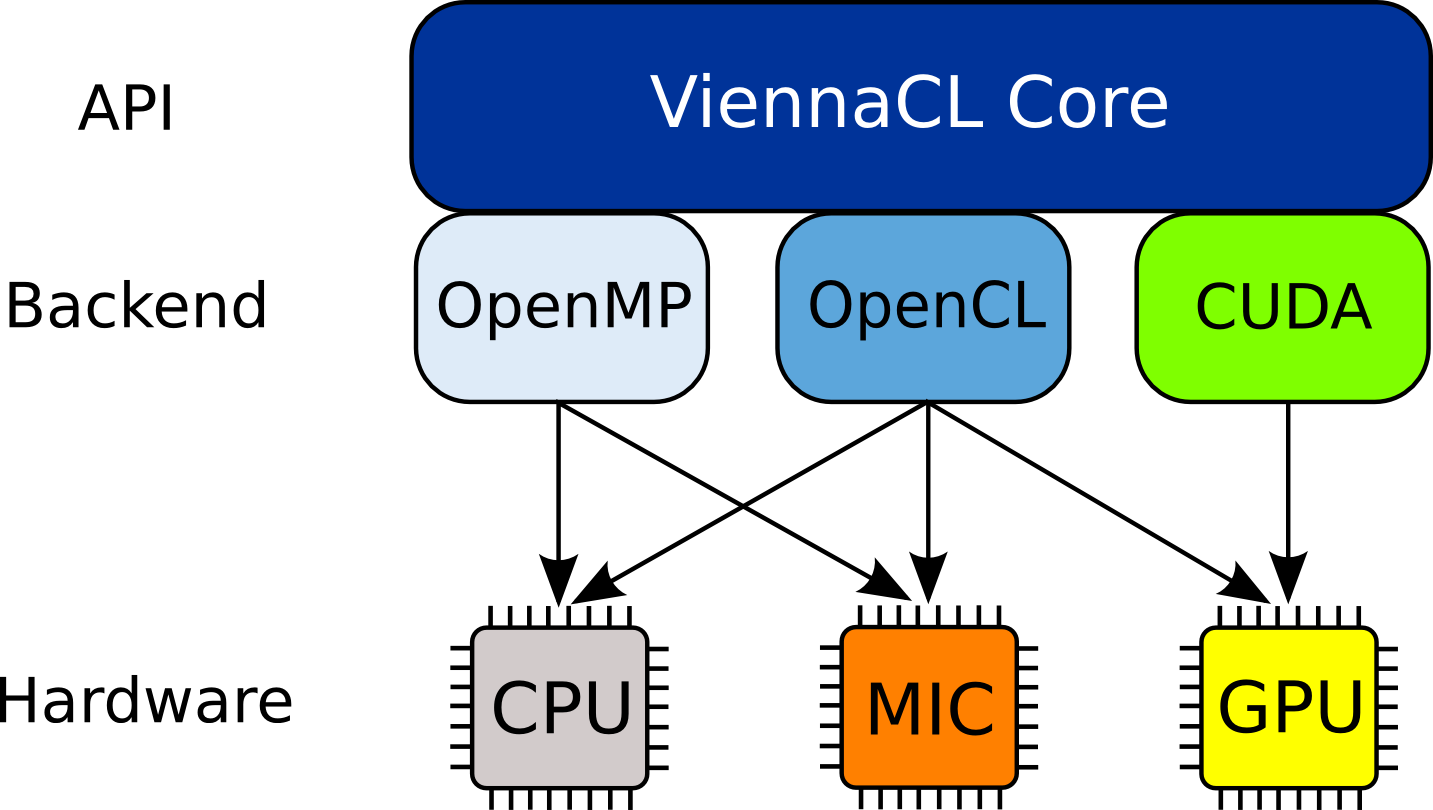
\includegraphics[width=0.4\textwidth]{figures/ViennaCL-arch.png}
  \end{flushright}

  \vspace*{-0.7cm}
  \begin{block}{Dissemination}
    \begin{itemize}
     \item Free Open-Source MIT (X11) License
     \item http://viennacl.sourceforge.net/
     \item 50-100 downloads per week
    \end{itemize}   
  \end{block}

  \begin{block}{Design Rules}
   \begin{itemize}
    \item Reasonable default values
    \item Compatible to Boost.uBLAS whenever possible 
    \item In doubt: clean design over performance
   \end{itemize}
  \end{block}

\end{frame}

%%%%%%%%


%%%%%%%%%%%%%%% Explain ViennaCL types here %%%%%%%%%%%%%%%%%%%%%%

\begin{frame}[fragile]
\frametitle{About ViennaCL}

 \begin{block}{Basic Types}
   \begin{itemize}
    \item scalar
    \item vector
    \item matrix, compressed\_matrix, coordinate\_matrix, ell\_matrix, hyb\_matrix
   \end{itemize}
 \end{block}

 \begin{block}{Data Initialization}
    \begin{itemize}
     \item Using viennacl::copy() 
    \item  { \black
  \begin{lstlisting}
     std::vector<double>      std_x(100);
   ublas::vector<double>    ublas_x(100);
viennacl::vector<double>      vcl_x(100);


for (size_t i=0; i<100; ++i){
    std_x[i] = rand();
  ublas_x[i] = rand();
    vcl_x[i] = rand();  //possible, inefficient
}
  \end{lstlisting} }

%   \item Reuse of C++ STL coding conventions
 \end{itemize}

 \end{block}
\end{frame}



\begin{frame}[fragile]
\frametitle{About ViennaCL}

 \begin{block}{Basic Types}
   \begin{itemize}
    \item scalar
    \item vector
    \item matrix, compressed\_matrix, coordinate\_matrix, ell\_matrix, hyb\_matrix
   \end{itemize}
 \end{block}

 \begin{block}{Data Initialization}
    \begin{itemize}
     \item Using viennacl::copy() 
    \item  { \black
  \begin{lstlisting}
     std::vector<double>      std_x(100);
   ublas::vector<double>    ublas_x(100);
viennacl::vector<double>      vcl_x(100);

/* setup of std_x and ublas_x omitted */

viennacl::copy(std_x.begin(), std_x.end(),
               vcl_x.begin());   //to GPU
viennacl::copy(vcl_x.begin(), vcl_x.end(),
               ublas_x.begin()); //to CPU
  \end{lstlisting} }

%   \item Reuse of C++ STL coding conventions
 \end{itemize}

 \end{block}
\end{frame}


\begin{frame}[fragile]
\frametitle{About ViennaCL}

 \begin{block}{Basic Types}
   \begin{itemize}
    \item scalar
    \item vector
    \item matrix, compressed\_matrix, coordinate\_matrix, ell\_matrix, hyb\_matrix
   \end{itemize}
 \end{block}

 \begin{block}{Data Initialization}
    \begin{itemize}
     \item Using viennacl::copy() 
    \item  { \black
  \begin{lstlisting}
     std::vector<std::vector<double> >    std_A;
   ublas::matrix<double>                ublas_A;
viennacl::matrix<double>                  vcl_A;

/* setup of std_A and ublas_A omitted */

viennacl::copy(std_A,
               vcl_A);    // CPU to GPU
viennacl::copy(vcl_A,
               ublas_A);  // GPU to CPU
  \end{lstlisting} }
 \end{itemize}

 \end{block}
\end{frame}







\begin{frame}[fragile]
\frametitle{Internals}

 \begin{block}{Vector Addition}
  \begin{lstlisting}
 x = y + z;
  \end{lstlisting}
 \end{block}

  %\pause

 \begin{block}{Naive Operator Overloading}
  \begin{lstlisting}
 vector<T> operator+(vector<T> & v, vector<T> & w);
  \end{lstlisting}

  %\pause

  \begin{itemize}
   \item t $\leftarrow$ y + z, x $\leftarrow$ t
   %\pause
   \item Temporaries are extremely expensive! 
  \end{itemize}
 \end{block}

   %\pause

 \begin{block}{Expression Templates}
  \begin{lstlisting}
 vector_expr<vector<T>, op_plus, vector<T> >
 operator+(vector<T> & v, vector<T> & w) { ... }

 vector::operator=(vector_expr<...> const & e) {
   viennacl::linalg::avbv(*this, 1,e.lhs(), 1,e.rhs());
 }
  \end{lstlisting}
  \vspace*{0.5cm}

 \end{block}

\end{frame}



\begin{frame}[fragile]
\frametitle{Internals}

 \begin{block}{Vector Addition}
  \begin{lstlisting}
// x = y + z
void avbv(...) {
  switch (active_handle_id(x))
  {
    case MAIN_MEMORY:
      host_based::avbv(...);
      break;
    case OPENCL_MEMORY:
      opencl::avbv(...);
      break;
    case CUDA_MEMORY:
      cuda::avbv(...);
      break;
    default: 
      raise_error();
  }
}
\end{lstlisting}
  \begin{itemize}
   \item Memory buffers can switch memory domain at runtime
  \end{itemize}

 \end{block}

\end{frame}

\begin{frame}[fragile]
\frametitle{Internals}

 \begin{block}{Memory Buffer Migration}
  \begin{lstlisting}
  vector<double> x = zero_vector<double>(42);

  memory_types src_memory_loc = memory_domain(x);
  switch_memory_domain(x, MAIN_MEMORY);

  /* do work on x in main memory here */

  switch_memory_domain(x, src_memory_loc);
\end{lstlisting}

  \begin{center}
    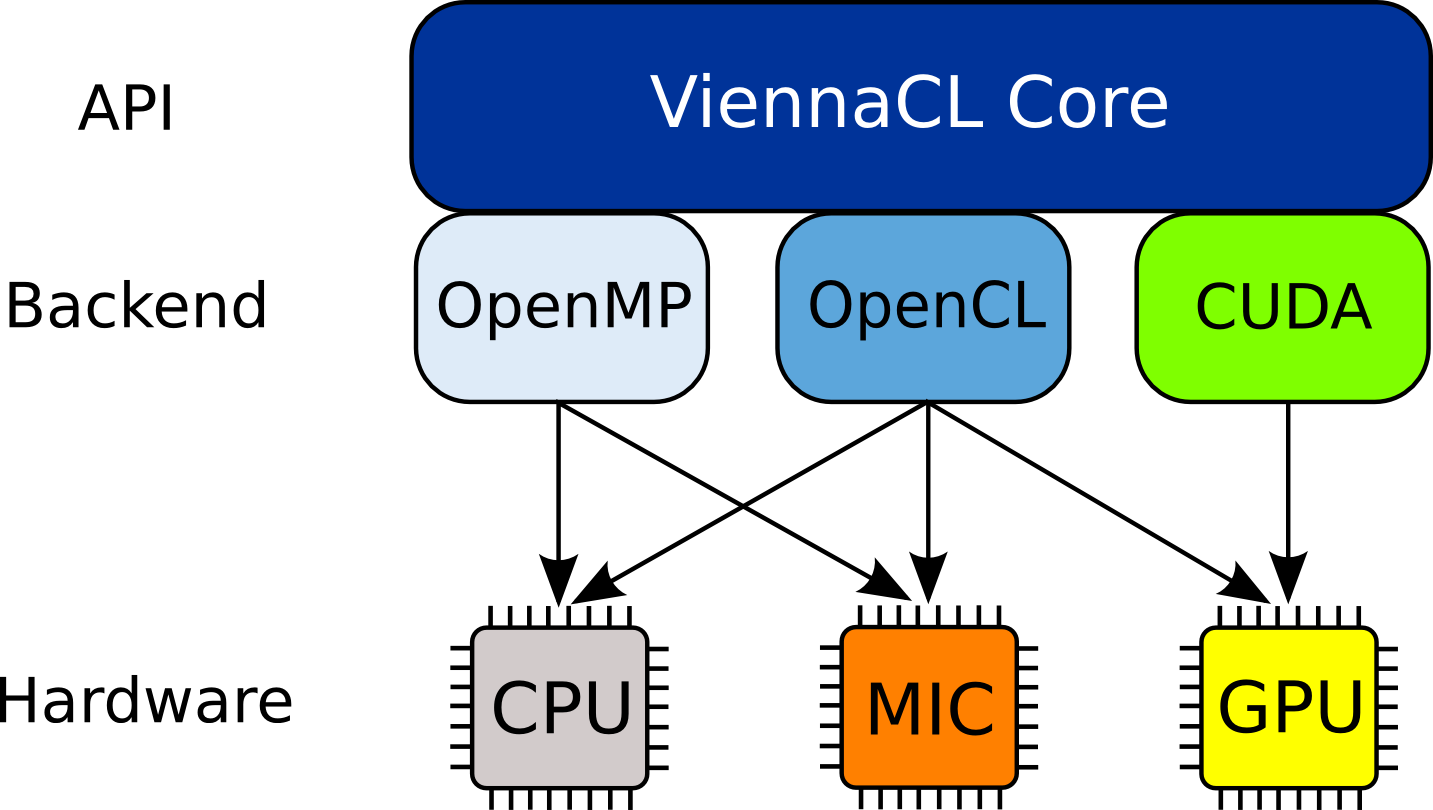
\includegraphics[width=0.6\textwidth]{figures/ViennaCL-arch.png}
  \end{center}
 \end{block}

\end{frame}




\begin{frame}[fragile]
\frametitle{Internals}

 \begin{block}{Generalizing compute kernels}
  \begin{lstlisting}
  // x = y + z
  __kernel void avbv(
    double * x,

    double * y,

    double * z, uint size)
{
  i = get_global_id(0);
  for (size_t i=0; i<size; i += get_global_size())
    x[i] = y[i] + z[i]; 

}
  \end{lstlisting}
 \end{block}

 \vspace*{1.5cm}
\end{frame}



\begin{frame}[fragile]
\frametitle{Internals}

 \begin{block}{Generalizing compute kernels}
  \begin{lstlisting}
  // x = a * y + b * z
  __kernel void avbv(
    double * x,
    double a,
    double * y,
    double b,
    double * z, uint size)
{
  i = get_global_id(0);
  for (size_t i=0; i<size; i += get_global_size())
    x[i] = a * y[i] + b * z[i]; 

}
  \end{lstlisting}
 \end{block}

 \vspace*{1.5cm}
\end{frame}


\begin{frame}[fragile]
\frametitle{Internals}

 \begin{block}{Generalizing compute kernels}
  \begin{lstlisting}
  // x[4:8] = a * y[2:6] + b * z[3:7]
  __kernel void avbv(
    double * x, uint off_x,
    double a,
    double * y, uint off_y,
    double b,
    double * z, uint off_z, uint size)
{
  i = get_global_id(0);
  for (size_t i=0; i<size; i += get_global_size())
    x[off_x + i] = a * y[off_y + i] + b * z[off_z + i]; 

}
  \end{lstlisting}
 \end{block}

 \vspace*{1.5cm}
\end{frame}



\begin{frame}[fragile]
\frametitle{Internals}

 \begin{block}{Generalizing compute kernels}
  \begin{lstlisting}
  // x[4:2:8] = a * y[2:2:6] + b * z[3:2:7]
  __kernel void avbv(
    double * x, uint off_x, uint inc_x,
    double a,
    double * y, uint off_y, uint inc_y,
    double b,
    double * z, uint off_z, uint inc_z, uint size)
{
  i = get_global_id(0);
  for (size_t i=0; i<size; i += get_global_size())
    x[off_x + i * inc_x] =  a * y[off_y + i * inc_y]
                          + b * z[off_z + i * inc_z]; 
}
  \end{lstlisting}
 \end{block}

  \begin{block}{}
   \begin{itemize}
    \item No penalty on GPUs because FLOPs are for free
   \end{itemize}
  \end{block}

\end{frame}








%\begin{frame}{Benchmarks}
%  \begin{center}
%   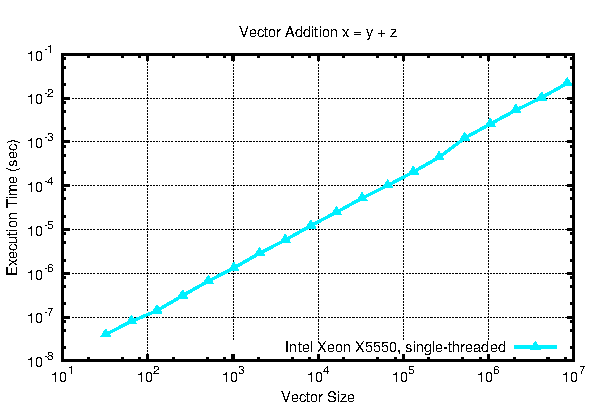
\includegraphics[width=0.95\textwidth]{figures/vector-timings-1}
%  \end{center}
%\end{frame}

%\begin{frame}{Benchmarks}
%  \begin{center}
%   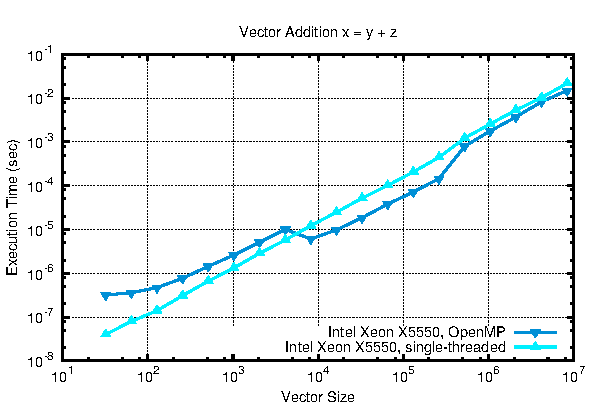
\includegraphics[width=0.95\textwidth]{figures/vector-timings-2}
%  \end{center}
%\end{frame}

%\begin{frame}{Benchmarks}
%  \begin{center}
%   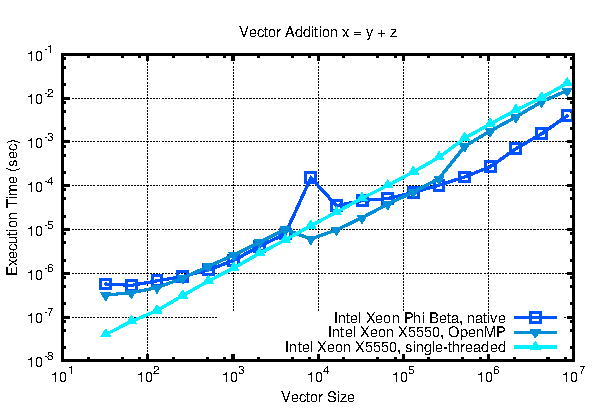
\includegraphics[width=0.95\textwidth]{figures/vector-timings-3}
%  \end{center}
%\end{frame}

%\begin{frame}{Benchmarks}
%  \begin{center}
%   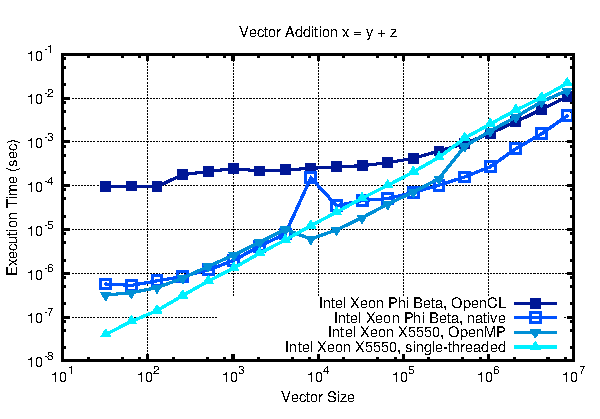
\includegraphics[width=0.95\textwidth]{figures/vector-timings-4}
%  \end{center}
%\end{frame}

%\begin{frame}{Benchmarks}
%  \begin{center}
%   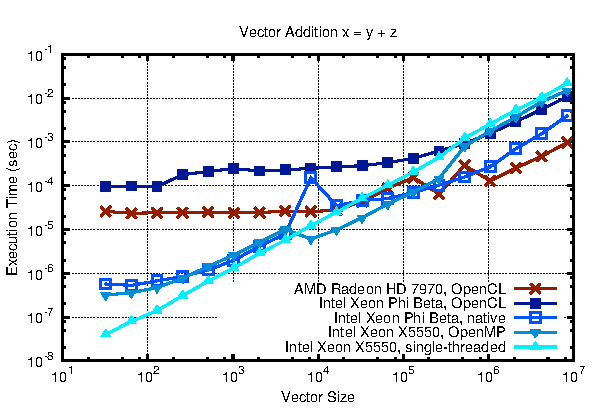
\includegraphics[width=0.95\textwidth]{figures/vector-timings-5}
%  \end{center}
%\end{frame}

%\begin{frame}{Benchmarks}
%  \begin{center}
%   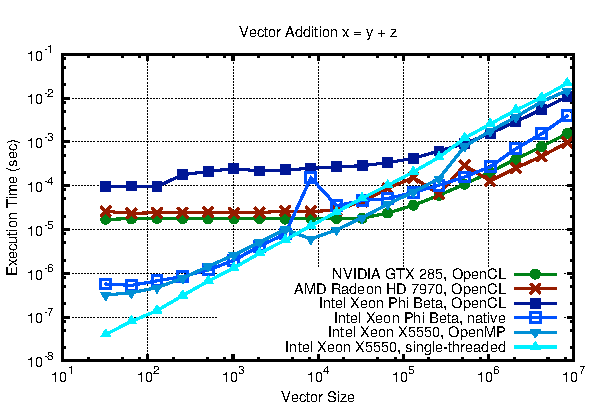
\includegraphics[width=0.95\textwidth]{figures/vector-timings-6}
%  \end{center}
%\end{frame}

\begin{frame}{Benchmarks}
  \begin{center}
   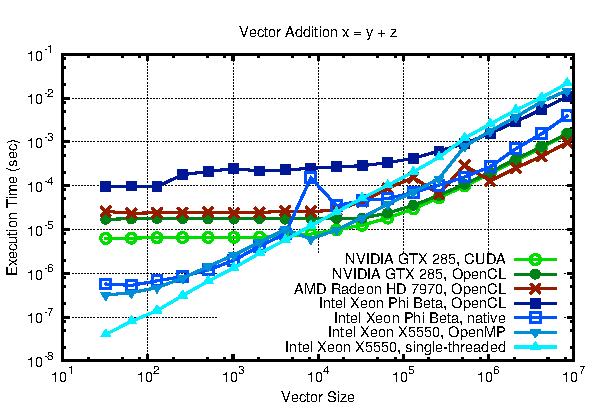
\includegraphics[width=0.95\textwidth]{figures/vector-timings-7}
  \end{center}
\end{frame}

%%

%\begin{frame}{Benchmarks}
%  \begin{center}
%   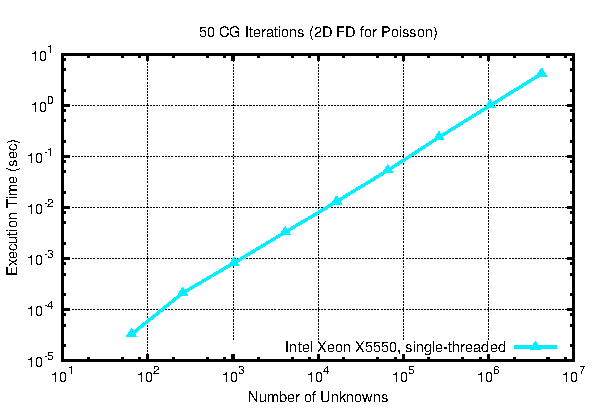
\includegraphics[width=0.95\textwidth]{figures/cg-timings-1}
%  \end{center}
%\end{frame}

%\begin{frame}{Benchmarks}
%  \begin{center}
%   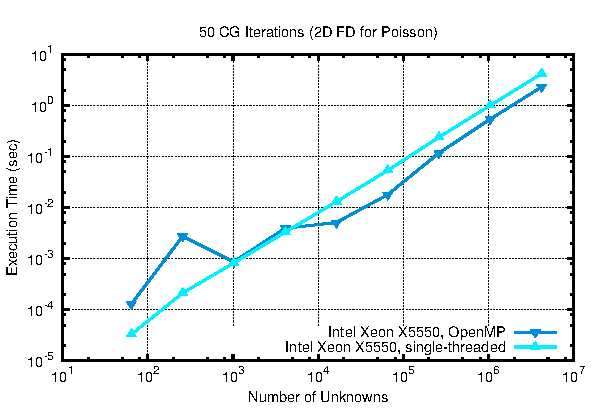
\includegraphics[width=0.95\textwidth]{figures/cg-timings-2}
%  \end{center}
%\end{frame}

%\begin{frame}{Benchmarks}
%  \begin{center}
%   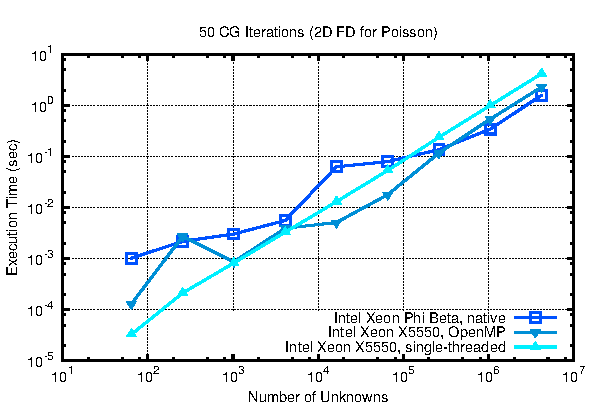
\includegraphics[width=0.95\textwidth]{figures/cg-timings-3}
%  \end{center}
%\end{frame}

%\begin{frame}{Benchmarks}
%  \begin{center}
%   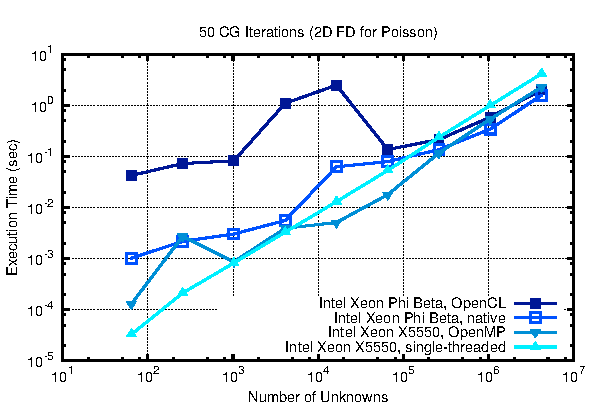
\includegraphics[width=0.95\textwidth]{figures/cg-timings-4}
%  \end{center}
%\end{frame}

%\begin{frame}{Benchmarks}
%  \begin{center}
%   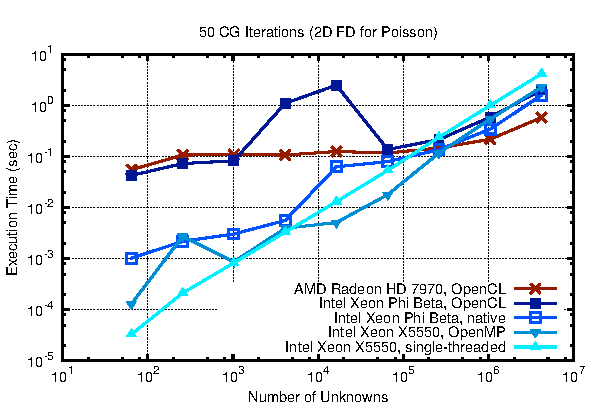
\includegraphics[width=0.95\textwidth]{figures/cg-timings-5}
%  \end{center}
%\end{frame}

%\begin{frame}{Benchmarks}
%  \begin{center}
%   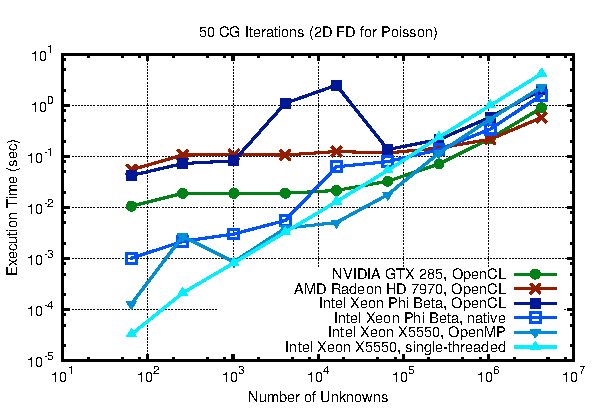
\includegraphics[width=0.95\textwidth]{figures/cg-timings-6}
%  \end{center}
%\end{frame}

\begin{frame}{Benchmarks}
  \begin{center}
   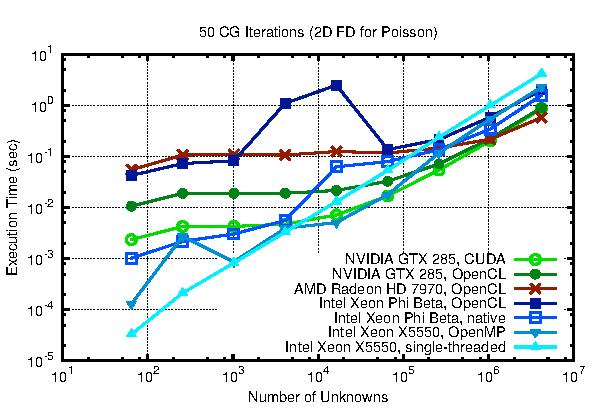
\includegraphics[width=0.95\textwidth]{figures/cg-timings-7}
  \end{center}
\end{frame}


\begin{frame}{Benchmarks}

 \begin{block}{Matrix-Matrix Multiplication}
  \begin{itemize}
   \item Autotuning environment 
   \item 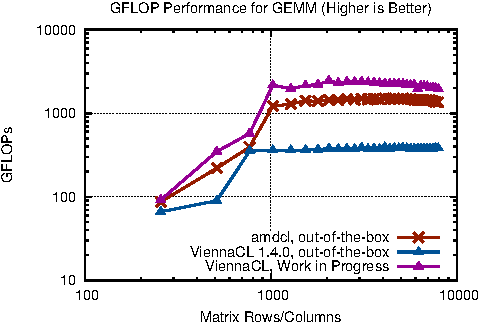
\includegraphics[width=0.85\textwidth]{figures/gemm3.pdf}
   \item \centering (AMD Radeon HD 7970, single precision)
  \end{itemize}

 \end{block}

\end{frame}






\begin{frame}{Acknowledgements}

 \begin{minipage}{0.5\textwidth}
  \begin{block}{Contributors}
    \begin{itemize}
     \item Thomas Bertani
     \item Evan Bollig
     \item Philipp Grabenweger
     \item Volodymyr Kysenko
     \item Nikolay Lukash
     \item G\"unther Mader
     \item Vittorio Patriarca
     \item Florian Rudolf
     \item Astrid Rupp
     \item Philippe Tillet
     \item Markus Wagner
     \item Josef Weinbub
     \item Michael Wild
    \end{itemize}
  \end{block}
 \end{minipage}
 \begin{minipage}{0.4\textwidth}
  
\includegraphics[width=0.65\textwidth]{figures/gsoc2011.png}
  \vspace*{0.2cm} \\
  
\includegraphics[width=0.65\textwidth]{figures/gsoc2012.png}
  \vspace*{0.2cm} \\
  
\includegraphics[width=0.65\textwidth]{figures/nvidia_logo_black.png}
  \vspace*{0.2cm} \\
  
\includegraphics[width=0.65\textwidth]{figures/amd-logo.png}
 \end{minipage}

\end{frame}




\begin{frame}{Summary}
 
 \begin{block}{High-Level C++ Approach of ViennaCL}
  \begin{itemize}
   \item Convenience of single-threaded high-level libraries (Boost.uBLAS)
   \item Header-only library for simple integration into existing code
   \item MIT (X11) license
   \item \centering http://viennacl.sourceforge.net/
  \end{itemize}
 \end{block}

 \begin{block}{Selected Features}
  \begin{itemize}
   \item Backends: OpenMP, OpenCL, CUDA
   \item Iterative Solvers: CG, BiCGStab, GMRES
   \item Preconditioners: AMG, SPAI, ILU, Jacobi
   \item BLAS: Levels 1-3
   \item 
  \end{itemize}
 \end{block}

\end{frame}
